% !TEX encoding = UTF-8
% !TEX TS-program = pdflatex
% !TEX root = ../apprendimento_automatico.tex
% !TEX spellcheck = it-IT
\section{Lezione 5 VC-Dimension e VC-Confidence}\label{lezione-5-vc-dimension-e-vc-confidence}

\subsection{Esempi di spazi delle ipotesi}\label{esempi-di-spazi-delle-ipotesi}

Seguono alcuni esempi di spazi per le ipotesi nei problemi di
apprendimento supervisionato, cioè quei problemi in cui si vuole
stabilire se un elemento \emph{x} appartiene o meno ad una classe.

\subsubsection{Iperpiani in R2}\label{iperpiani-in-r2}

\textbf{Iperpiano}: dato uno spazio a \emph{n}-dimensioni, un iperpiano
per quello spazio è un sottospazio di dimensione \emph{n-1}. Ad esempio gli
iperpiani in $R^2$ sono tutte le rette del piano.

Lavorando in $R^2$ lo spazio delle istanze è definito come:

$$
X = \{x | x \in R^2\}.
$$

Mentre lo spazio delle ipotesi è dato dalle dicotomie indotte da iperpiani in $R^2$, cioè da tutte le possibili divisioni del piano.

$$
H = \{f_{(w,b)}(x) | f_{(w,b)}(x) = sign(w \times x + b), w \in R^2, b \in R\}
$$

Così facendo vengono prese in considerazione tutte le rette che dividono
$R^2$ in due parti in modo che da una parte l'ipotesi valga 1 e dall'altra
-1.

\subsubsection{Dischi in R2}\label{dischi-in-r2}

Sempre in $R^2$ è possibile considerare come spazio delle ipotesi tutte le
dicotomie indotte da dischi in $R^2$ e centrati nell'origine.

$$
H = \{f_b(x) | f_b(x) = sign(||x||^2 - b), w \in R2, b \in R\}
$$

Il che vuol dire che all'interno del disco le ipotesi valgono -1 mentre
al di fuori valgono 1.

\subsubsection{\texorpdfstring{Congiunzione di \emph{m} letterali positivi}{Congiunzione di m letterali positivi}}\label{congiunzione-di-m-letterali-positivi}

Lo spazio delle istanze questa volta è dato da tutte le stringhe di \emph{m} bits

$$
X = \{s | s \in \{0,1\}^m\}
$$

Lo spazio delle ipotesi è dato da tutte le sentenze logiche che
riguardano i letterali positivi $l_1$,$l_2$,\ldots{},$l_m$ ($l_i$ è vero se
l'\emph{i}-esimo bit è 1) e che contengono solo l'operatore $\wedge$.

$$
H = \{ f_{(i_1,\ldots,i_j}(s) | f_{(i_1,\ldots,i_j}(s) \text{ equivale a } l_{i_1} \wedge l_{i_2} \wedge \ldots \wedge l_{i_j}, \{i_1\ldots{}i_j\} \text{ sottoinsieme di }  \{1..m\}\}
$$

\subsection{Misurare la complessità dello spazio delle ipotesi}\label{misurare-la-complessituxe0-dello-spazio-delle-ipotesi}

Considerato un determinato spazio delle ipotesi \emph{H}, questo
contiene sempre:

\begin{itemize}
\tightlist
\item
  L'\textbf{ipotesi più specifica}: ipotesi più stretta e consistente con
  i dati, nell'esempio del disco è il disco più stretto in grado di
  contenere tutti i punti negativi.
\item
  L'\textbf{ipotesi più generale}: quella più grande e consistente con i
  dati, sempre nell'esempio del disco, è quello del disco più grande
  possibile e che non contiene punti positivi.
\end{itemize}

\textbf{Shattering}: (frammentazione), dato \emph{S} sottoinsieme dello
spazio delle istanze, si dice che \emph{S} è frammentato dallo spazio
delle ipotesi \emph{H} se:

$$ 
\forall S' \in S, \exists h \in H, \text{ tale che } \forall x \in S, h(x) = 1 \text{ se e solo se } x \in S'.
$$

Cioè \emph{H} realizza tutte le possibili dicotomie di \emph{S}.

\emph{H} frammenta un certo insieme \emph{S} se è possibile trovare un
iperpiano \emph{h} che raccoglie tutti i punti dell'insieme \emph{S}. Ovvero per
tutte le dicotomie di \emph{S} esiste un iperpiano che riesce a
realizzarle.

\subsubsection{VC (Vapnik-Chervonenkis) Dimension}\label{vc-vapnik-chervonenkis-dimension}

La VC-Dimension è la dimensione di uno spazio delle ipotesi \emph{H}
definito su uno spazio delle istanze \emph{X} ed è data dalla
cardinalità del sottoinsieme più grande frammentato da \emph{H}.

\begin{align*}
VC(H) &= max_{S \subseteq X} |S| \text{ tale che \emph{H} frammenta } S  \\
&= \infty \text{se S non è limitato}
\end{align*}


Ad esempio nello spazio delle ipotesi dato dagli iperpiani su $R^2$:

Se nello spazio delle istanze ho 2 punti, questo viene frammentato da
\emph{H}, perché posso sempre trovare una retta che riesce a realizzare
tutte le possibili dicotomie di due punti su un piano.

Se nello spazio delle istanze ho 3 punti, riesco comunque a realizzare
tutte le dicotomie.

Se nello spazio delle istanze ho 4 punti qualsiasi non si riesce a
trovare un iperpiano che realizza la dicotonomia, quindi \emph{VC(H) =
3}.

Segue che, prendendo uno spazio delle ipotesi di cardinalità finita si
ha che:

$$
VC(H) \leq log_2(|H|)
$$

Questo perché per ogni \emph{S} frammentato da \emph{H}, abbiamo
$|H| \geq 2^{|S|}$,
cioè per ogni dicotomia in \emph{S} esiste un ipotesi in \emph{H} che la
realizza, ovvero devono essere disponibili in \emph{H} tante ipotesi
quanti sono le dicotomie in \emph{H}.

Scegliendo un \emph{S} tale che $|S| = VC(H)$, si
ottiene $|H| \geq 2^{|S|}$, prendendo
il logaritmo si trova quello che si stava cercando, ovvero $VC(H) \leq log_2(|H|)$.

\textbf{Dal libro}:

Se un dataset contiene \emph{N} elementi, questi \emph{N} elementi
possono essere etichettati con degli 0 e 1 in $2^N$ modi diversi.

Se per ognuno di questi modi è possibile trovare un ipotesi $h \in H$
che separa tutte le istanze negative da quelle positive allora si dice
che \emph{H} frammenta il dataset \emph{N}. 
Il che vuol dire che il dataset \emph{N} può essere appreso con un errore empirico nullo.

Il massimo numero di punti che possono essere frammentati da \emph{H} è
detto \emph{VC(H)} e fornisce una misura della capacità di \emph{H}.

\subsection{Bound sull'errore di generalizzazione}\label{sec:vcc}

Considerando un problema di apprendimento binario, con:

\begin{align*}
\text{Training set }S &= \{(x_i,y_i), \ldots (x_N, y_N)\} \\
\text{Spazio delle ipotesi } H &=\{h_\theta(x)\} 
\end{align*}

Supponendo di avere un algoritmo di apprendimento \emph{L} che
restituisce l'ipotesi $h_{\theta*}$ che minimizza l'errore empirico su
\emph{S} espresso come $errore_S(h_\theta(x))$.

È possibile derivare un bound (limite superiore) per l'errore ideale o
errore di generalizzazione, valido con probabilità \emph{(1 - $\sigma$)} con
$\sigma$ piccolo a piacere:

$$
errore_D(h_\Theta(x)) \leq  errore_S(h_{\theta}(x)) + g(N, VC(H), \sigma)
$$

Il primo termine $errore_S(h_{\theta}(x))$ dipende dall'ipotesi restituita
dall'algoritmo di apprendimento \textit{L}.

Il secondo termine $g(N, VC(H), \sigma)$ non dipende da \emph{L}, ma dal
numero di esempi di training utilizzati (inversamente proporzionale),
dalla \emph{VC-dimension} (direttamente proporzionale) e dalla
confidenza, ovvero dal termine $\sigma$.

Questo termine viene anche chiamato \textbf{VC-confidence} e risulta essere monotono rispetto al rapporto
$\frac{VC(H)}{N}$.

\textbf{Morale della favola}: la VC-Dimension sottostima con confidenza $\sigma$ l'errore ideale.

\subsection{Structural Risk Minimization (SRM)}\label{sec:srm}

Approccio per la scelta dello spazio delle ipotesi proposto da Vapnik
che cerca di trovare un compromesso tra l'errore empirico e la
VC-Confidence.

Si considerano spazi delle ipotesi sempre più piccoli $H_1 \subseteq H2 \subseteq \ldots \subseteq H_n$ tali che $ VC(H_1) \leq VC(H_2) \leq \ldots \leq VC(H_n)$

Si seleziona lo spazio delle ipotesi $H_i$ che ha il valore del bound
sull'errore di generalizzazione più piccolo. ovvero la VC-Dimension minore.

\begin{figure}[htbp]
\centering
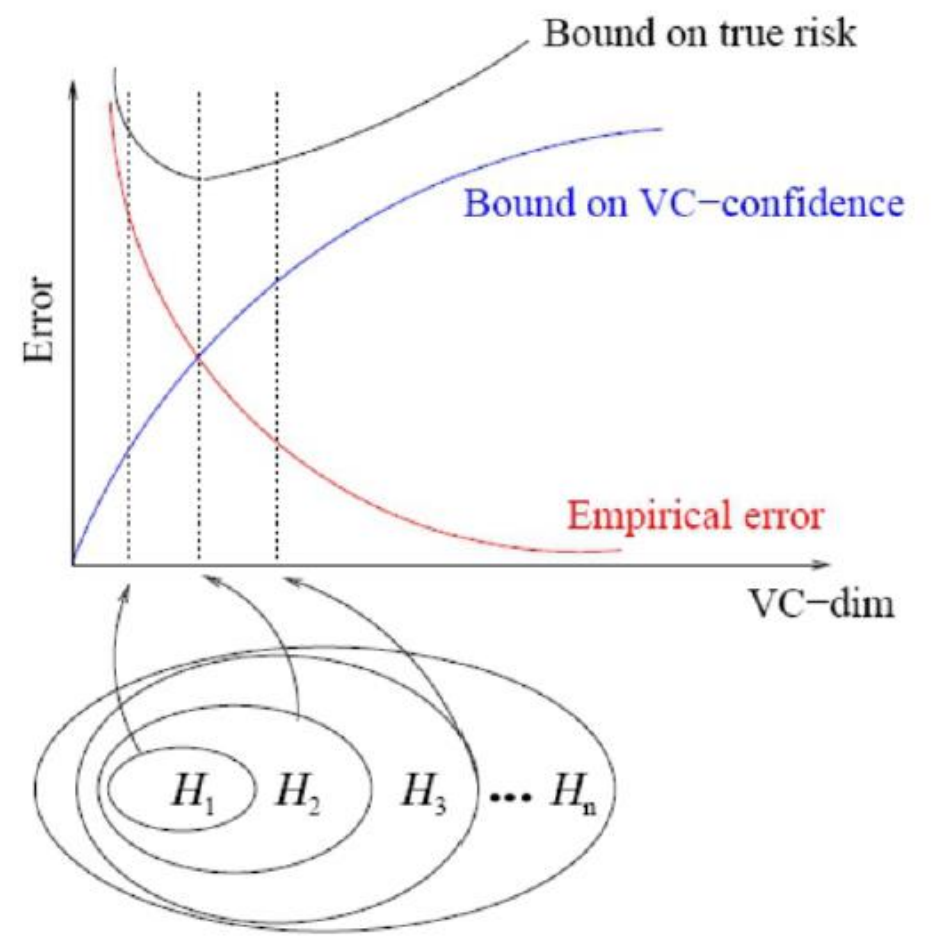
\includegraphics[width=0.5\textwidth]{./notes/immagini/l5-srm.png}
\caption{Structural Risk Minimization}
\end{figure}
